\chapter{Introducción a la filosofía de la ciencia}
\label{cha:filosofiaciencia}

Estás en una carrera de Ciencias, rodeado de Científicos que hacen cosas
científicas, pero ¿qué es exactamente la ciencia?
¿Por qué la astronomía es una ciencia pero la astrología no?
¿A qué se dedican los científicos?
¿Es el método científico la única forma de hacer ciencia?
¿Un conocimiento científico es más confiable que un conocimiento no científico?
Todas estas preguntas son las que discuten los filósofos de la ciencia, y tratar
de responderlas y debatirlas nos brinda un mejor panorama de la naturaleza misma
de esta disciplina.

Para este capítulo ten en cuenta que las herramientas de la filosofía no son
las mismas que las de la ciencia.
La principal diferencia con los otros cursos de nuestra carrera es que aquí no
hay una respuesta definitiva a las preguntas que se plantean, y que el progreso
se logra mediante la discusión y la dialéctica: alguien propone una idea, otro
la critica, y así sucesivamente hasta llegar a un consenso, aunque este no sea
definitivo.

\section{Los orígenes de la ciencia}
\label{sec:losorigenesdelaciencia}

Para ponernos en contexto es importante conocer los orígenes de la ciencia, así
será más fácil entender por qué funciona como lo hace en la actualidad.

\subsection*{La ciencia en la antigüedad}
\label{sub:cienciaenlaantiguedad}
Desde la antigua Grecia, los filósofos se preguntaban por las causas del mundo.
Tal es el caso de \index{Aristóteles}{Aristóteles} (384--322 a. C.), quien
propuso muchas teorías físicas basándose en acertijos conceptuales y
razonamientos lógicos, pero sin experimentación ni
observación\cite{sep-aristotle}.
Su \index{física}{\emph{física}} se basaba en la idea de que la naturaleza busca
siempre la economía y la perfección; por ende sus teorías no fueron muy
acertadas.
Por ejemplo, él afirmaba que los cuerpos caen con una velocidad proporcional a
su peso.
A esta cosmovisión se le conoce como \terminology[aristotelismo]{aristotelismo},
y fue la base del conocimiento científico hasta el siglo \textsc{xvii}.

Parte central del aristotelismo fue la \index{teoría!geocéntrica}%
{teoría geocéntrica}, introducida por \index{Ptolomeo}{Ptolomeo} (90--168
d. C.). Esta teoría postula que la Tierra es el centro del universo y que todos
los demás cuerpos celestes giran alrededor de ella.

\begin{figure}[ht]
    \centering
    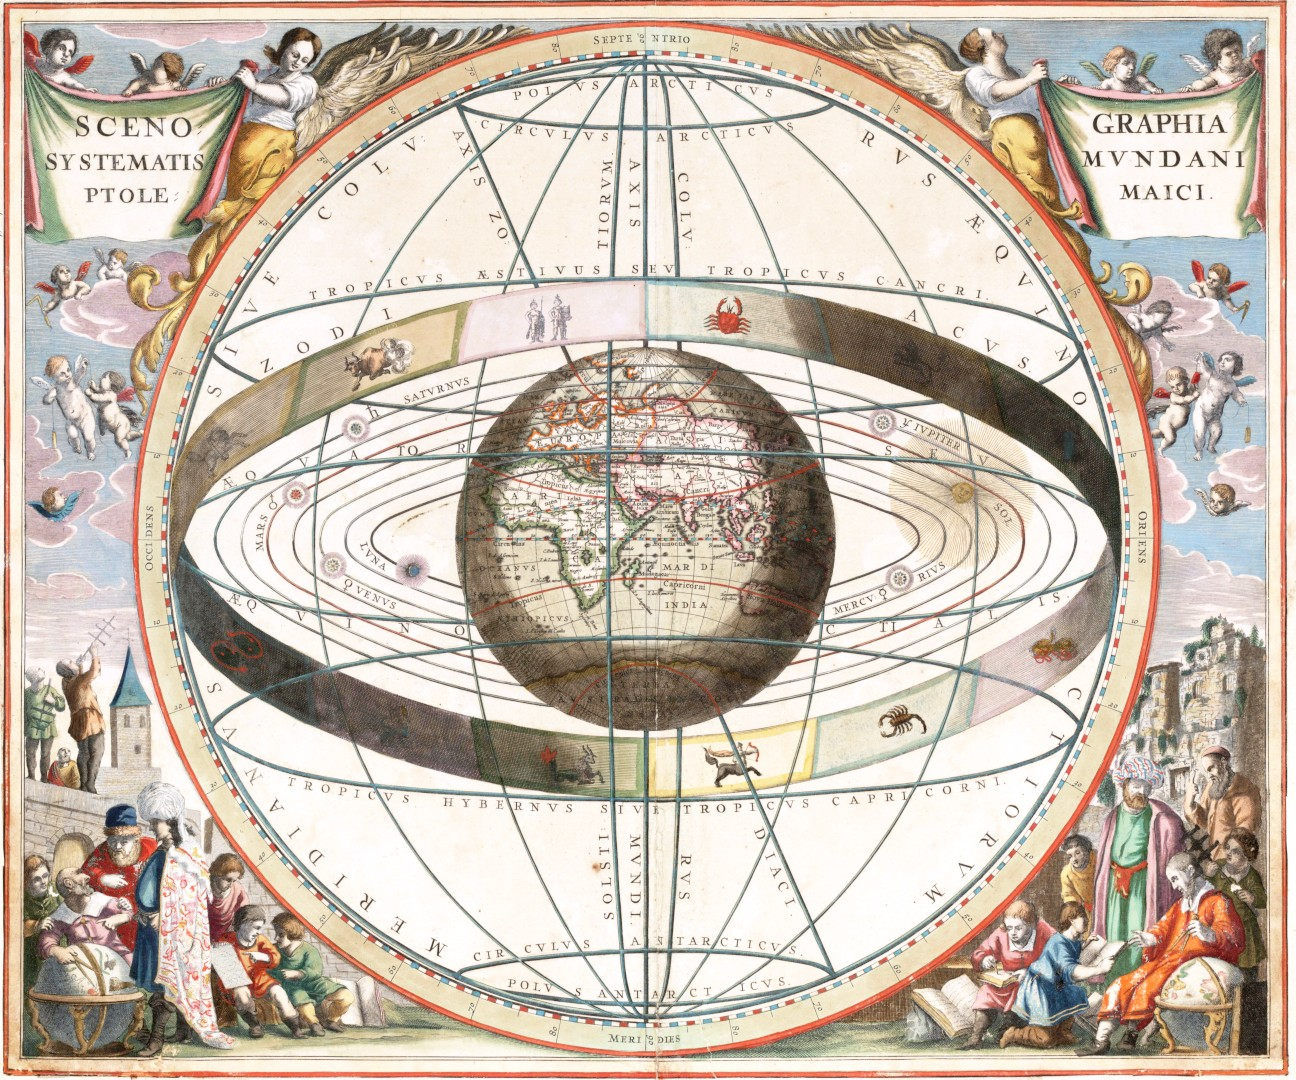
\includegraphics[width=0.8\linewidth]{img/Cellarius_ptolemaic_system}
    \caption{El sistema ptolemaico, en el que la Tierra es el centro del
        universo. Crédito: Loon, J. van (Johannes), aprox. 1611--1686.}
    \label{fig:ptolemaico}
\end{figure}

\subsection*{La revolución científica}
\label{sub:larevolucioncientifica}
Fue hasta 1542 cuando el canónigo católico \index{Copérnico, Nicolás}%
{Nicolás Copérnico} (1473--1543) se atrevió a desafiar el aristotelismo
publicando su libro \emph{De revolutionibus orbium coelestium} (Sobre las
revoluciones de las esferas celestes), en el que propone que el Sol está fijo en
el centro del universo y que los planetas giran alrededor de él, dando lugar así
a la \index{teoría!heliocéntrica}{\emph{teoría heliocéntrica}}.

La teoría no fue bien recibida por la Iglesia, ni aún cuando su autor la dedicó
al Papa Pablo \textsc{iii}.
Más bien fue vetada de 1616 a 1835, pero en solo cien años se había convertido
en la teoría dominante gracias a los trabajos de \index{Galileo Galilei}{Galileo
    Galilei} (1564--1642) y \index{Johannes Kepler}{Johannes Kepler}
(1571--1630).
Kepler descubrió que los planetas se mueven en órbitas elípticas y no circulares
como creía Copérnico, y así resolvió el problema de la posición de Marte en el
cielo nocturno.
En cambio, Galileo apuntó su telescopio al cielo y descubrió que Júpiter tiene
cuatro lunas, que la Luna tiene montañas y cráteres, y que el Sol tiene manchas
entre otras cosas.

Galileo también hizo importantes contribuciones en otras áreas de la ciencia;
descubrió la \emph{ley de caída de los cuerpos}, que dice que todos los cuerpos
caen con la misma aceleración.
Según relata su discípulo Vivianni, esto lo demostró dejando caer dos bolas de
diferente peso desde lo alto de la Torre inclinada de Pisa
\cite{Viviani+2019+1+94}.
Hasta entonces la lógica aristotélica era suficiente para explicar el mundo, la
experimentación era considerada una actividad de segunda clase, y las
matemáticas servían para describir objetos ideales pero no la realidad.
Galileo cambió todo esto, y por ello se le considera el primer científico
moderno.
Desafortunadamente, Galileo fue condenado por la Inquisición en 1633 por
defender a la teoría heliocéntrica, que para entonces era considerada herética
por contradecir la creación del mundo descrita en la Biblia.
Él pasó el resto de su vida bajo arresto domiciliario y se convirtió así también
en el ejemplo más famoso del conflicto entre ciencia y religión.

Luego de la muerte de Galileo, la ciencia entró en una etapa de rápido avance.
\index{Descartes, René}{René Descartes} (1596--1650), con su
\terminology[mecanicismo]{mecanicismo}, propuso que el universo es como una
maquinaria de reloj en la que todo puede explicarse en términos del movimiento
y colisión de partículas.
Asimismo, en su \emph{Discurso del método} (1637) propuso que la ciencia debe
basarse en la razón y no en la autoridad, y que la experimentación y la
observación son las herramientas más importantes para el científico.

Por su parte, \index{Newton, Isaac}{Isaac Newton} (1643--1727) propuso sus tres
leyes del movimiento y la ley de la gravitación universal, que explica la
atracción entre los cuerpos celestes.
Su obra maestra intitulada \emph{Philosophiae Naturalis Principia Mathematica}
(Principios matemáticos de la filosofía natural) se publicó en 1687, y fue el
marco teórico de referencia para la ciencia durante los siguientes 200 años.
Esta teoría sería extendida por muchos otros científicos para explicar más
fenómenos, como la mecánica de fluidos o la teoría electromagnética.

\begin{figure}[ht]
    \centering
    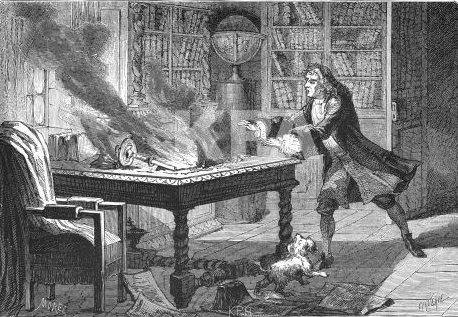
\includegraphics[width=0.8\linewidth]{img/Isaac_Newton_laboratory_fire}
    \caption{Isaac Newton en su laboratorio.
        Su mascota \emph{Diamond} tiró una vela sobre una mesa de papeles,
        quemando varios años de trabajo en el proceso.
        Crédito: Morel / Dominio público.
    }

\end{figure}

Durante un par de siglos se consideró que la teoría de Newton era esencialmente
correcta, y que los científicos sólo necesitaban rellenar meros detalles
técnicos para completar el cuadro.

\subsection*{La ciencia moderna}
\label{sub:lacienciamoderna}
En 1859, \index{Darwin, Charles}{Charles Darwin} (1809--1882) publicó su libro
\emph{El origen de las especies}, en el que propone la teoría de la evolución
mediante la selección natural.
Antes de esto ya se sabía que las especies cambian con el tiempo si se
seleccionan artificialmente a los individuos más aptos para la reproducción.
Así, en la agricultura y la ganadería se habían obtenido nuevas variedades de
plantas y animales más aptas para el consumo humano.
Darwin propuso que este mismo proceso ocurre en la naturaleza, donde las
especies co-evolucionan con su entorno y se adaptan a él.

A mediados del siglo \textsc{xix} el físico escocés \index{Maxwell, James}%
{James Maxwell} (1831--1879) descubrió que la luz es una onda electromagnética
que se propaga a la velocidad de la luz, unificando así las teorías de la
electricidad y el magnetismo.
Esto fue un gran avance, pero también un problema, pues las ecuaciones de
Maxwell entran en conflicto con la mecánica Newtoniana cuando se consideran
altas velocidades.
El final del siglo \textsc{xix} y el principio del \textsc{xx} fueron testigos
de invenciones increíbles como el teléfono, la radio, y el avión, pero también
de descubrimientos científicos que cimbraron la visión mecanicista del mundo.
En 1905, \index{Einstein, Albert}{Albert Einstein} (1879--1955) publicó su
\emph{teoría de la relatividad especial}, en la que propuso que el tiempo y el
espacio son relativos, y que la velocidad de la luz es la misma para todos los
observadores.

Por otro lado, apareció el problema de la \emph{radiación del cuerpo opaco}, que
desafiaba la física clásica al intentar comprender cómo un objeto caliente emite
radiación electromagnética.
Las predicciones clásicas indicaban que bajo ciertas condiciones este emitiría
radiación infinita, en clara contradicción con las observaciones experimentales.
Este problema fue resuelto por \index{Planck, Max}{Max Planck} (1858--1947) en
1900, quien propuso que la energía se emite en paquetes discretos llamados
\emph{cuantos}, dando origen a la \index{mecánica cuántica}{mecánica cuántica}.

En conjunto, la teoría de la relatividad y la mecánica cuántica revolucionaron
la física y la ciencia en general, disminuyendo la confianza en la teoría de
Newton y en el método científico clásico.
Ambas teorías son tan extrañas como exitosas, y han sido confirmadas por miles
de experimentos, pero aún así son difíciles de entender y de aceptar.

En 1936, \index{Turing, Alan}{Alan Turing} (1912--1954) publicó su artículo
\emph{On computable numbers, with an application to the Entscheidungsproblem},
en el que propuso un concepto matemático que eventualmente se convertiría en el
fundamento teórico de la computadora programable.
Su trabajo fue fundamental para el desarrollo de las computadoras y de la
computación moderna, sembrando la posibilidad de analizar a-priori el
comportamiento de un programa de computadora y sus limitaciones, aunque pasarían
varios años antes de que esto se hiciera realidad con la primera computadora
electrónica \emph{ENIAC} (Electronic Numerical Integrator and Computer) en 1946.

\begin{figure}[ht]
    \centering
    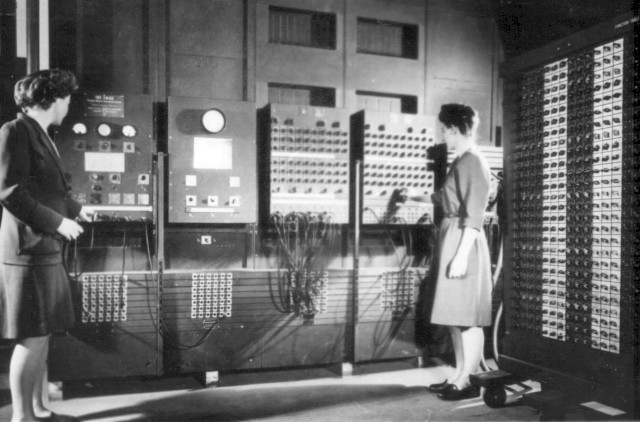
\includegraphics[width=0.8\linewidth]{img/Two_women_operating_ENIAC}
    \caption{Dos mujeres operando la computadora ENIAC.
        Crédito: U.S. Army Photo / Dominio público.
    }
\end{figure}

Para 1953, \index{Watson, James}{James Watson} (1928--) y
\index{Crick, Francis}{Francis Crick} (1916--2004) descubrieron la estructura
del ácido desoxirribonucleico (ADN), la molécula que contiene la información
genética de los seres vivos, dando inicio a la \index{biología!molecular}%
{biología molecular} que estudia los procesos biológicos en términos de las
moléculas que los componen.
Esta disciplina se ha desarrollado rápidamente gracias a la computación, que
permite simular y analizar los procesos biológicos a nivel molecular.
En 2003 se completó el \index{Proyecto Genoma Humano}{Proyecto Genoma Humano},
que consistió en secuenciar el ADN de un ser humano, y que ha permitido
entender mejor las enfermedades genéticas y desarrollar nuevos tratamientos
médicos.

\begin{figure}[ht]
    \centering
    \includegraphics[height=0.618\textheight]%
    {img/60_Jahre_DNA_01.jpg}
    \caption{Réplica del modelo de ADN de Watson y Crick.
        Crédito: Museum für Naturkunde Berlin.}
\end{figure}

\subsection*{La ciencia contemporánea}
El siglo \textsc{xx} fue testigo de la creación o formalización de disciplinas
como \index{economía}{economía}, \index{antrolopogía}{antropología},
\index{sociología}{sociología}, \index{psicología}{psicología}, y
\index{lingüística}{lingüística}.
En general, estas disciplinas se basan en el método científico, pero no son
ciencias naturales.
Por ejemplo, la sociología estudia la sociedad y la cultura, pero es mayormente
una ciencia observacional, pues no se pueden hacer experimentos con sociedades
humanas.

La tendencia actual es hacia la interdisciplinariedad, es decir, la
colaboración entre diferentes disciplinas para resolver un problema.
Una de estas ciencias artificiales que ha contribuido significativamente a
lograr esto es la \index{computación}{computación}, que estudia los fundamentos,
limitaciones y aplicaciones de la programación de computadoras.
La computación ha permitido simular y analizar fenómenos complejos que antes
eran inaccesibles.
Por ejemplo, la climatología estudia el clima de la Tierra, y para ello
simula el comportamiento de la atmósfera mediante modelos computacionales.
Estos métodos computacionales cuestionan la naturaleza misma de la ciencia.
¿Es válido un conocimiento científico que no se basa en la experimentación ni
en la observación, pero que es capaz de predecir el comportamiento de un
fenómeno observado?

Asimismo, la computación ha permitido el desarrollo de la inteligencia
artificial, que estudia la creación de máquinas inteligentes.
Esto ha llevado a la creación de programas de computadora que pueden jugar
ajedrez, conducir automóviles, diagnosticar enfermedades, pero más importante
para nuestra discusión, que hacer ciencia.
Estos programas de computadora se han usado exitosamente para descubrir
exoplanetas, predecir la estructura de proteínas, y descubrir nuevos materiales
entre otras cosas.
¿Se puede considerar \emph{conocimiento científico} a los resultados de estos
programas de computadora?

\section{Qué es la Ciencia}
\label{sec:queeslaciencia}

La ciencia intenta explicar, entender y predecir el mundo, pero también la
religión, la astrología, e incluso otras disciplinas como historia y filosofía.
La diferencia está en los métodos, a saber: la experimentación, observación y
construcción de teorías, pero definir exactamente qué es la ciencia es un
problema que ha ocupado a los filósofos durante siglos, y se conoce como el
\terminology[problema!demarcación]{problema de demarcación}.
A continuación veremos algunas propuestas que han surgido para resolver este
problema.

\subsection*{El empirismo}
\label{sub:elemprismo}
Durante la revolución científica, el filósofo inglés \index{Bacon, Francis}%
{Francis Bacon} (1561--1626) propuso, de forma retrospectiva, que la ciencia
debe basarse en la experimentación y la observación en su libro \emph{Novum
    Organum} (1620).
Para Bacon, la ciencia debe ser \emph{inductiva}, es decir, que debe partir de
muchas observaciones particulares para llegar a una conclusión general.
Esta es la idea central del \terminology[empirismo]{empirismo}.
Así, cuando un empirista quiere entender algún fenómeno natural como la
combustión de la madera, debe observar muchos casos particulares de madera
quemándose para llegar a una conclusión general sobre el fenómeno.

Esto tiene mucho sentido para nosotros, pero en la antigüedad se creía que el
conocimiento se podía obtener mediante la razón y la lógica, y la
experimentación era relegada a un segundo plano.

Sin embargo este método tiene un problema: ¿cuántas observaciones son
suficientes para llegar a una conclusión general?
Si un turista visita a México, y más concretamente visita Tijuana, El Pinacate,
Cuatro Ciénegas, Real de Catorce, y el Paseo del Viejo Oeste de Durango, ¿puede
decir que todo México es un desierto?
¿Cuántos lugares debe visitar para poder decir que México es un país desértico?
¿Qué pasa si visita El Cañón del Sumidero, la Ciudad de México, o el Nevado de
Toluca?

\begin{figure}[ht]
    \centering
    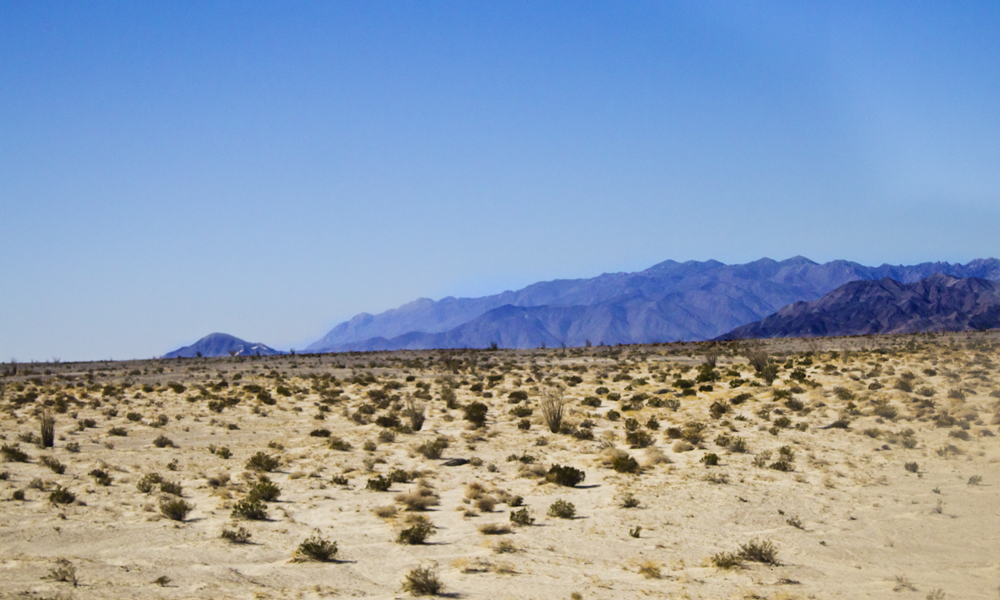
\includegraphics[width=\linewidth]{img/Desierto_de_San_Luis_Rio_Colorado}
    \caption{El desierto de San Luis Río Colorado, Sonora, es una prueba
        contundente de que México es un país desértico.
        Crédito: Wikimedia Commons / CC BY-SA 4.0.}
\end{figure}

Quizás para este momento estés pensando que podemos corregir este problema si
además de observaciones también exigimos experimentos.
Desafortunadamente, esto no es suficiente, pues los experimentos no siempre dan
cuenta de las \emph{variables ocultas}.
Por ejemplo, si dejamos caer un martillo y una pluma desde la misma altura, el
martillo caerá más rápido, y estarías tentado a decir que los objetos pesados
caen más rápido que los ligeros.
Sin embargo, si hacemos el experimento en el vacío, veremos que ambos caen con
la misma velocidad.
Esto es porque nuestro experimento no tomó en cuenta la resistencia del aire,
que es una variable oculta.
Este experimento al vacío ya fue llevado a cabo durante la misión
\emph{Apollo 15} en 1971, cuando el astronauta \index{David Scott}{David Scott}
\href{https://youtu.be/Oo8TaPVsn9Y}{ dejó caer una pluma y un martillo} en la
superficie lunar como homenaje a Galileo.

Si los experimentos no son suficientes, al menos podrías argumentar que por lo
menos sí son necesarios para hacer ciencia.
Esto tampoco es así, pues hay disciplinas que claramente son científicas pero
que no se basan en la experimentación, como es la astronomía.
Entonces, si la experimentación no es necesaria ni suficiente para describir a
un conocimiento como científico, ¿qué es lo que sí lo hace científico?

\subsection*{El falsacionismo}
\label{sub:elfalsacionismo}
El filósofo \index{Popper, Karl}{Karl Popper} (1902--1994) intentó abordar este
problema de distinguir la ciencia de la no-ciencia mediante el
\terminology[falsacionismo]{falsacionismo}.
Según Popper, una teoría científica es aquella que, al menos en principio, puede
ser refutada mediante la experimentación.
Por ejemplo, la ley de caída de los cuerpos de Galileo es una teoría científica
porque si el día de hoy quisieras refutarla, bastaría con soltar dos bolas de
diferente peso desde una altura y ver que caen con distinta aceleración (siempre
que tomes en cuenta la resistencia del aire y otros factores).
Probablemente nunca lograrás refutarla, pero la mera posibilidad de hacerlo es
lo que cuenta; esta es la característica fundamental de una teoría científica.

La idea central del falsacionismo es muy simple y tiene mucho sentido,
después de todo, ¿qué sentido tiene una teoría que no se puede generalizar?
Encuentra una anomalía o contraejemplo y toda la teoría se cae.
Aquí además es importante considerar que en nuestra búsqueda de anomalías
\emph{la ausencia de evidencia no es evidencia de ausencia}.
Es decir, si no encuentras una anomalía no significa que no exista, sino que
no la has encontrado.
Así, mientras hayas intentado encontrarla y fracasado en el intento, tu teoría
es científica según Popper.

¿Y cómo es que esto nos permite distinguir entre ciencia y no-ciencia?
Consideremos las \terminology[pseudociencia]{pseudociencias}, que son
disciplinas que se hacen pasar por ciencia pero que no lo son.
La astrología tiene cierto parecido con la astronomía porque ambas estudian los
cuerpos celestes, pero la astrología es universalmente considerada una creencia
supersticiosa.
¿Puede el falsacionismo ayudarnos a distinguir entre la astronomía y la
astrología?
Veamos: los astrónomos hacen predicciones suficientemente vagas como para que
siempre sean ciertas, y cuando no lo son, simplemente inventan una explicación
ad-hoc para justificarlas, como por ejemplo, que su predicción no se cumplió
porque la persona no se leyó el horóscopo en el momento adecuado.
Entonces la astrología no es científica porque no puede ser refutada, y por lo
tanto es una pseudociencia.
¿Qué hay de la astronomía?
Los astrónomos hacen predicciones muy específicas, como por ejemplo, que el
próximo eclipse solar será visible en toda América del Norte el 8 de abril de
2024.
Si este eclipse no ocurre, entonces la teoría de la astronomía se cae, y por lo
tanto es una teoría científica.
Así ha ocurrido con muchas predicciones astronómicas, como la predicción de
\index{Edmond Halley}{Edmond Halley} (1656--1742) de que el cometa que lleva su
nombre volvería a ser visible desde la Tierra en 1758, lo cual ocurrió en la
fecha predicha.

Entonces, ¿es el falsacionismo la solución al problema de demarcación?
No tan rápido; hay dos problemas con esta propuesta.
En primera, suena muy extraño decir que los científicos \emph{inventan}
teorías de la nada y sólo se dedican a refutarlas.
Ciertamente eso no ocurre en la práctica; generalmente los científicos se
dedican a \emph{construir} teorías de forma paulatina, y sólo cuando se
encuentran varias anomalías es que se dedican a refutarlas.
En efecto, el segundo problema es que en la práctica no es fácil ni conveniente
rechazar una teoría científica solo porque se encontró una anomalía.

Un ejemplo muy delicioso ocurrió en 1963, cuando un estudiante de Tanzania
llamado \index{Mpemba, Erasto}{Erasto Mpemba} (1950--) descubrió durante una
clase de hacer helados que el agua caliente se congela más rápido que el agua
fría.
Más tarde, en 1969, publicó un artículo en el que describía su
descubrimiento\cite{E+B+Mpemba_1979}, pero los científicos no le creyeron porque
contradecía la teoría de la termodinámica.
¿Abandonaron los científicos la teoría de la termodinámica cuando vieron que
Mpemba tenía razón?
Por supuesto que no; en su lugar, se dedicaron a buscar una explicación a este
fenómeno en el marco de la teoría de la termodinámica, y en 2017 dos equipos
independientes de científicos publicaron artículos en los que explicaban el
fenómeno.


\section{Los métodos científicos}
\label{sec:losmetodoscientificos}

\section{Las revoluciones científicas}
\label{sec:lasrevolucionescientificas}

\section{Crítica a la ciencia}
\label{sec:criticaalaciencia}
